%\begin{savequote}[8cm]
%\textlatin{Neque porro quisquam est qui dolorem ipsum quia dolor sit amet, consectetur, adipisci velit...}

%There is no one who loves pain itself, who seeks after it and wants to have it, simply because it is pain...
%  \qauthor{--- Cicero's \textit{de Finibus Bonorum et Malorum}}
%\end{savequote}

\chapter{\label{ch:1-intro} Latent Dirichlet Allocation for the Unsupervised Discrimination of ATAC-seq Experiments}
%\chapter{Machine learning, or something like that...}

\minitoc

\providecommand{\tightlist}{%
  \setlength{\itemsep}{0pt}\setlength{\parskip}{0pt}}

%\section{Motivation}

\section{Introduction} \label{ch4:intro}



\subsection{Hyperparameters}

\section{Methods} \label{ch4:methods}


\subsection{Single Cell ATAC-seq Dataset Generation} \label{methods:sc_ds}

A single cell dataset was compiled from data generated in \textcite{Buenrostro2015} for three cell types: K562, GM12878, and H1ESC. These cell types were selected as a minimal subset which represents maximal diversity in accessible chromatin within the larger dataset. 

For each labelled cell type, we collected accession numbers within the NCBI sequence read archive. These include records SRR1780163 through SRR1780354 (K562), SRR1779683 through SRR1779778 (GM12878), and SRR1779589 through SRR1779683 (H1ESC). Sequencing reads were merged and adapters were trimmed with cutadapt v 2.10 using the following adapter seqences ({\tt -a CTGTCTCTTATACACATCT -A CTGTCTCTTATACACATCT}) \cite{Martin2011}. Quality of the merged dataset was verified with fastqc and aligned to hg19 using bowtie2 \cite{Andrews2010, Langmead2013}. Cell specific barcodes were added to the resulting alignment file within the {\tt CB} tag using pySam \cite{Heger2009}. Peak calling was performed using macs2 and lanceotron using default parameters \cite{Gaspar2018, Hentges2021} as detailed in \autoref{ch4:method_peaks} and count matrices were constructed as detailed in \autoref{ch4:method_cistopic}.

\subsection{Construction of Pseudo-bulk ATAC-seq Dataset}

In order to construct a pseudo-bulk dataset, entries for each of the single cells were merged into a single alignment file. Cell barcodes were replaced with a cell-type marker and peak calling was similarly conducted with macs2 and lanceotron \cite{Gaspar2018, Hentges2021}.

\subsection{Peak Calling from Coverage Data} \label{ch4:method_peaks}

We compare two methods of peak calling.

A public implementation of the LanceOTron can be found at \url{https://github.com/chris1221/lanceotron}. LanceOTRon relies on a pre-trained neural network. We use the supplied weights in \url{wide_and_deep_fully_trained_v5_03.h5} along with the standard scaler values from the same implementation. We allow the network to identify candidate peaks and assign a peak score, thresholding our selected peaks on a peak score of at least 0.5 as in the implemention of LanceOTron at \url{https://lanceotron.molbiol.ox.ac.uk/}.


\subsection{Running LDA with cisTopic} \label{ch4:method_cistopic}

We use the implementation of \gls{lda} in cisTopic \cite{BravoGonzalez-Blas2019}. cisTopic is intended for use on single cell ATAC-seq experiments, however the input format is amenable to any quantative data observed on a cell by region basis. To construct the input data to cisTopic, we construct a bespoke pipeline that firstly calls peaks from ATAC-seq experiments, and secondly harmoises these peaks while constructing a count matrix. A count matrix is a sparse matrix where the rows are cells, or in the case of this thesis, cell types, and the columns are regions.



\subsection{Bayesian Hyper-parameter Optimization} \label{ch4:hyper}

\gls{lda} requires a set of three hyper-parameters to be supplied, alpha, beta, and the number of topics. This chapter investigates applications of LDA to problems of several scales, so the choice of hyper-parameters is not easily chosen, at least in an unbiased way. We approach this issue by using a Bayesian Optimization approach to learn the best set of hyper parameters for a given set of ATAC-seq experiments. We wrote a typical cisTopic analysis in python via rpy2 ({\tt https://rpy2.github.io/doc/latest/html/index.html}) and used the BayesianOptimization library ({\tt https://github.com/fmfn/BayesianOptimization}) to optimize a target function for a given set of hyper-parameters. This task was facilitated by the use of Dask to compute several hundred possible combinations simultaneously \cite{Rocklin2015}. The target function to optimise is based on the specific application, as discussed in \autoref{ch4:results} section.

\subsection{Bulk LDA (BLDA) Method}

The BLDA method is a small extension to cisTopic which aims to incorporate a proxy of how accessible each peak region is in a particular experiment. This makes it in some ways more similar to the traditional approach to LDA within natural language processing, which gives an integer value for the number of times a particular word appears in a text. To create the RPKM normalized count matrix and run the inference, we use functions from the blda python package available on Github at \url{https://github.com/Chris1221/blda}. \todo{Link the snakemake pipeline minus the data.} The construction of the count matrix requires linked coverage files and their associated peak calls. The pipeline is agnostic to the type of coverage file (either BAM files or RPKM normalised bigWig tracks can be provided) and peak calls can be made by any software which outputs delineated, non-overlapping genomic regions. Hyper-parameter optimization is conducted according to \Cref{ch4:hyper} and a modified version of cisTopic is run using {\tt rpy2}. The modification to cisTopic, found at \url{https://github.com/Chris1221/cisTopic}, relaxes a constraint to provide the {\tt lda} package's collapsed Gibb's sampler with a binary sparse matrix. Several other functions from the cisTopic function are applicable directly to the situation of bulk LDA after the data has been altered. 

\subsection{Computing the average fold enrichment of topics for groups} \label{methods:average_fc}

To get a measure for the number of topics to use in a particular model, we compute the average fold enrichment. This is done with a two step process. First, a one-tailed student's T test is performed for each of the grouping of cells. The cells are split into one of the cell types, with the remainder forming the comparison group. The null hypothesis here is that the means do not differ, or that the comparison group is significantly smaller than the group under question. The P values are corrected for the number of comparisons using Bonferroni correction (multiplying by the number of effective tests, which in this case is the number of tests) and the significant associations are reported. Second, the differences in the estimated means are divided to form a fold change metric amongst the subset of significant topic associations. We take the median of these values to form the average fold change metric for a particular set of topics being modelled. The median is selected to avoid extreme results overly biasing the statistic.


\section{Results} \label{ch4:results}

LDA has previously been shown to be highly effective at detecting true patterns in shared accessibility in single cell data. Here, I create a datset of known cell types in order to set baseline expectations about the capabilities of LDA in a single cell system before moving on to studying bulk samples.

\subsection{Bulk LDA recapitulates patterns from single cell ATAC-seq}

I generate a dataset of three labelled cell types, as per \Cref{methods:sc_ds}. This dataset comprises three cell types which have substantial differences in their accessible DNA.  K562 is an erythro-leukemic cell model of chronic myelogenous leukemia from a fifty three year old female donor \cite{Lozzio1975}. GM12878 is an \gls{ebv} immortalized B-lymphocyte cell line cultured from a female member of the international HapMap project CEPH panel \cite{Belmont2005}. Finally, H1ESC are a human embryonic stem cell line collected from a healthy male donor of unknown age \cite{Thomson1998}. 

The dataset comprises 96 GM12878 cells with a total of 1928090 reads, 96 H1ESC cells with 4192100 reads in total, and 192 K562 cells from two biological replicates with a total of 5269388 reads.

We generate coverage tracks for the merged single cell dataset using deepTools and peaks are called using both MACS2 and LanceOTron as per \Cref{ch4:method_peaks} \cite{Ramirez2014}. MACS2 identifies 10,075 statistically significant peak regions, while MACS2 finds 12,994, 8337 of which are common between the two approaches.  

\subsubsection{Identifying differentially accessible peaks with EdgeR} \label{ch4:edgeR}

The R package {\tt edgeR} is used to set a baseline expectation for differentially accessible regions of the genome between the clusters. {\tt edgeR} is selected as it was recently shown to have the overall highest sensitivity for identifying differential peaks from properly normalized ATAC-seq data. We took the single cell dataset and created a count matrix with all true counts across different cells. We inputted these into edgeR and estimated dispersion coefficients as recommended in the tutorial, fitting a generalised linear model according to the true cell identities which assume are known in this case. We identify the top 100 differentially accessible regions based on this analysis, and use these to study the results from our topic modelling approaches.

\begin{figure}
  \centering
  \includegraphics[width=\textwidth]{plot/ch4/sim_ll_surface.pdf}
  \caption{Hyperparameter log-likelihood surface for two hyperparameters.}
  \label{fig:llhood_surfacea_simulation}
\end{figure}

We investigate topic modelling in three separate scenarios. Firstly, we run cisTopic as intended, using the single cell data. Secondly, we create pseudo-bulk alignment files for each of the clusters and run cisTopic normally. Thirdly, we adapt cisTopic to accept normalized read count. This will allow us to validate our baseline assumption that LDA is able to capture similar information within bulk sequencing experiments.

\subsubsection{LDA captures realistic regulatory patterns in known single cell systems} \label{ch4:sc}

For the first case, we model the system of 384 cells with 4, 5, 6, 7, and 8 topics to assess the best biological fit to the system. For each pre-set number of topics, hyper parameters are selected using Bayesian optimization. The best value for $\alpha$ was not well estimated, with considerable noise and no clear peak; this is in contrast to the $\beta$ value, which showed higher log-likelihoods at higher values approaching 1 (\Cref{fig:sc_opt_params}). Consistent with this, a high value is selected for $\beta$ in each case. $\beta$ controls the number of regions loaded to a topic. With a number of cells much larger than the number of topics, especially in the present scenario, a high value of $\beta$ represents a prior on more regions loaded to each of the small number of topics. This indicates that a relatively high number of regions are differentially accessible between the different cluster. The relatively uncertain distribution of alpha log-likelihoods represents an ambiguity in the likelihood from different Dirichlet distributions. Draws with a low alpha tend to represent topic loadings which are specific to individual cells, and accordingly the flat likelihood surface may indicate that there are multiple ways of assigning the topics to cells with relatively equal likelihoods.

\todo{The alpha is off on \Cref{fig:sc_topics}, and I want to add labels to the K562 versus H1ESC and GM cells.}

\begin{figure}
  \centering
  \includegraphics[width=\textwidth]{plot/ch4/sc_opt_params}
  \caption{Single cell log likelihood for different values of the topic modelling hyper-parameters $\alpha$ and $\beta$ for various numbers of topics being modelled.}
  \label{fig:sc_opt_params}
\end{figure}

We investigate the loading of these topics on each of the cells in the collection (\Cref{fig:sc_topics}). As the number of topics modelled increases, some cell systems split more readily than others. H1ESC, for instance, has two enriched topics in even the smallest four topic model. For each of the number of topics, we calculate the median fold enrichment (\Cref{methods:average_fc}) and find that five and six topics produce very similar median fold enrichments (5.81 versus 5.82 respectively). To reduce the complexity of the model, and acknowledging that a model with more parameters will tend to fit data better, we choose the study the case with five topics.  

\begin{figure}
  \centering
  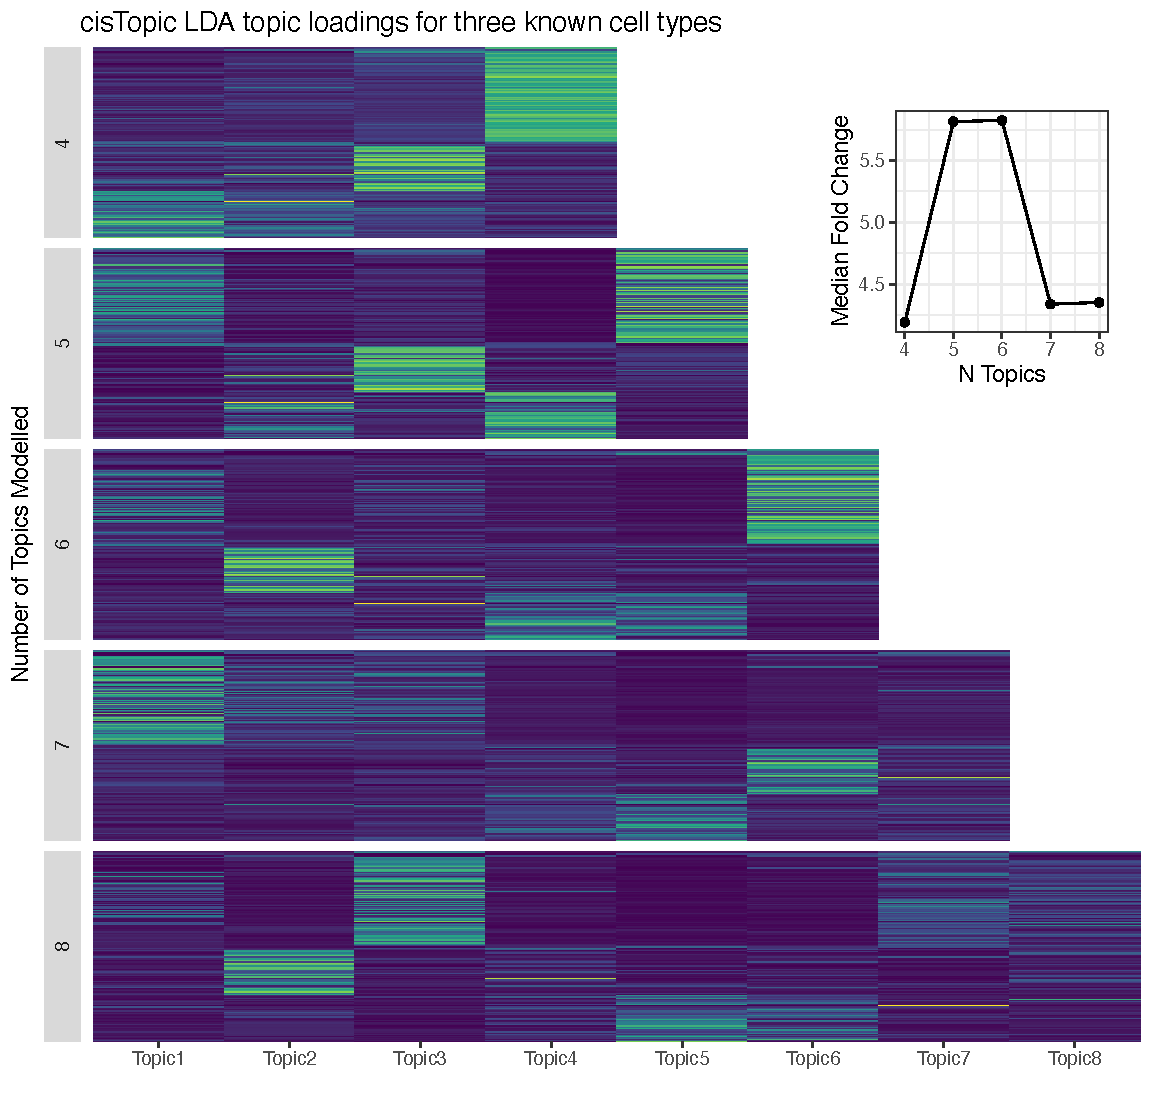
\includegraphics[width=\textwidth]{plot/ch4/sc_topics.pdf}
  \caption{Topic loadings for 4, 5, 6, 7, and 8 topic instances of the LDA inference procedure using optimal hyperparamters as decided in \Cref{fig:sc_opt_params}. Inset shows average fold change amungst enriched topics for each of the number of topics modelled. Enriched topics are identified by a one-tailed student's $t$ test for difference between a known cell cluster and the remainder of cells.} 
  \label{fig:sc_topics}
\end{figure}

\paragraph{Choice of peak caller influences the inference of topic loadings}

We additionally investigate the role that peak calling has on the inference of topics. 

Peaks were called with Macs2 instead of LanceOTRon, resulting in a larger number of peaks identified in general, with 4657 being uniquely identified by Macs2 (\Cref{fig:sc_macs2}A). We repeated the above analysis, including the hyper parameter search, topic inference, and calculation of median fold enrichment was conducted using MACS2 instead of LanceOTron, as detailed in \Cref{ch4:method_peaks}. Several differences are apparent in both the optimized hyper-parameters and the inferred topic loadings (\Cref{fig:sc_macs2}). Slight bias towards lower $\alpha$ values is observed in this dataset, and the same trend towards prefering higher values of $\beta$ is replicated here \Cref{fig:sc_macs2}B, C. However, when looking at the inferred topics, we find lower median fold enrichment in general (\Cref{fig:sc_macs2}D, E). From this we conclude that LanceOTron has identified a more specific set of accessible regions for the purposes of this study, and use it in all analyses going forward. 

\begin{figure}
  \centering
  \includegraphics[width=\textwidth]{plot/ch4/sc_macs2.pdf}
  \caption{Analysis of single cell dataset with peaks called by MACS2. A. The number of peak calls made by both callers, with their overlapping portion displayed in the center of the Venn diagram. B. Likelihood surface for the optimization of the $\alpha$ hyper-parameter. C. Likelihood surface for the optimization of the $\beta$ hyper-parameter. D. Median fold enrichment for topics inferred under optimal hyper-parameters. E. Inferred topic loadings on single cells using optimal hyper-parameters.}
  \label{fig:sc_macs2}
\end{figure}

LDA produces both a distribution of topic loadings on cells as well as topic loadings on regions. In order to identify regions putatively identified with the cell types through the topic loadings, a decision must be made about how to discretise the continuous loadings to a set of enriched regions. The cisTopic package accomplishes this by fitting a gamma distribution to the topic loadings, and identifying regions within the top user-defined percentile of this distribution. By default, this is set to the top 5\% of the distribution. Here we investigate how to set this parameter value and the influence it has on the resulting post-hoc analyses. 


\todo{Motif analysis here. Feather databse is still downloading so wait for it.}

\paragraph{Enrichment of differentially accessible regions within identified topics}

To assess whether the identified topic loadings represent similar trends to the baseline differential accessibility analysis, we fit a gamma distribution to the shape of each topic loading and take the top 2.5 percentile of the distribution as representative so-called "keywords" or key regions. We use bedtools to overlap these key regions with the 100 differentially accessible regions from the {\tt edgeR} analysis and find that 61 of the 100 regions are shared with the top 415 selected key regions (\Cref{table:sc_t5_over}). Given that there are 10074 regions in total, this represents a significant ($P<0.00001$, $\chi^2 = 827.33$) enrichment of differentially expressed regions in the selected regions from the LDA procedure.


\begin{table}
  \centering
  \begin{tabular}{l|l|l}
  Topic & Total Selected Regions & Intersecting Regions  \\ 
  \hline
  1     & 104                    & 15                    \\
  2     & 3                      & 0                     \\
  3     & 194                    & 29                    \\
  4     & 3                      & 1                     \\
  5     & 111                    & 19                   
  \end{tabular}
  \caption{Five topic single cell inferred topic loadings and the proportion of their selected regions which overlap 100 established differentially accessible regions. Overall, 61 of the 100 regions were found in the top 415 regions.}
  \label{table:sc_t5_over}
  \end{table}

\subsubsection{Extending LDA to Pseudo-bulked Single Cells}

We investigate whether the approach implemented in cisTopic is appropriate for use in bulk ATAC-seq experiments. This change represents a deviation in the intended system for the approach. Practically, the difference between the single cell case and the bulk one is the difference between a wide, sparse count matrix and a dense one with fewer observations. An attractive property of using Gibb's sampling to infer the posterior cell-topic distribution is its ability to efficiently deal with sparsity in the region-topic distribution. However, it is not clear to what degree this sparsity is a requirement for the procedure to obtain biologically relevant topics, each representing a proxy of co-accessible regulatory elements. In this section, I take the well-characterized single cell dataset from the previous section and study the analogous bulk sequencing case by artificially creating bulk samples from the individual known cell types. We denote these new bulk cells as pseudobulked samples.

We combine all reads from each known cell type into pseudo-bulked alignment files using pySam. Peak calling is performed separately on each of the pseudo-bulked samples using LanceOTron, as described in the single cell case. We additionally explore the role of thresholding on LanceOTRon peak calls by creating a subset of calls with at least 0.5 peak score. This is a recommendation made by the web interface to the peak caller. Before thresholding, 517620, 395953, and 455886 peaks were identified in the H1ESC, GM12878, and K562 cells respectively. After merging, 1063153 regions were used for the complete analysis. After thresholding on a peak score of 0.5, 7524, 4945, and 6722 peaks were found in the GM12878, H1ESC and K562 cells respectively. After merging, there were 16210 regions in total used for the thresholded case. 

We take two approaches to constructing the count matrix. The first is the already described cisTopic method, where peak regions are merged and annotated by contributing cell types, leading to a binary sparse matrix where the entries $i, j$ represent overlapped peak $j$ in cell type $i$. We denote this case as "one-hot encoded" as the representation is analogous to one-hot encoding factor levels within a design matrix. This approach is justified with the single cell case as read depth is much lower per cell, and a quantification of relative read support for a particular peak region is highly variable. In the case of bulk ATAC-seq however, a difference in read support for different regions can imply varying degrees of accessibility, a key feature of closely related cell types or differentiation processes.  \todo{CITE THIS} To reflect this in the model, we propose an extension of the cisTopic method which we call bulk LDA (BLDA). In this extension, we normalize read counts according to the floor of their reads per kilobase pair and million reads (RPKM) normalized value, giving an integer value of effective number of times the "word", or region, is represented in the particular dataset. This approach has the advantage of incorporating quantitative information about differential peak strengths across experiments, and more closely mimics typical applications of LDA within natural language processing. Here we investigate whether the quantitative extension of cisTopic for bulk ATAC-seq is able to better recapitulate the single cell case.

\begin{table}
  \centering
  \begin{tabular}[t]{lrrr}
  \toprule
  Method & Number of topics & Best Alpha & Best Beta\\
  \midrule
  \cellcolor{gray!6}{One-hot encoding} & \cellcolor{gray!6}{4} & \cellcolor{gray!6}{123.68822} & \cellcolor{gray!6}{0.0382351}\\
  One-hot encoding & 5 & 466.58752 & 0.0665157\\
  \cellcolor{gray!6}{One-hot encoding} & \cellcolor{gray!6}{6} & \cellcolor{gray!6}{450.96735} & \cellcolor{gray!6}{0.0756824}\\
  One-hot encoding & 7 & 337.58572 & 0.0769945\\
  \cellcolor{gray!6}{One-hot encoding} & \cellcolor{gray!6}{8} & \cellcolor{gray!6}{100.35205} & \cellcolor{gray!6}{0.0872716}\\
  \addlinespace
  RPKM Normalization & 4 & 40.38505 & 0.2350854\\
  \cellcolor{gray!6}{RPKM Normalization} & \cellcolor{gray!6}{5} & \cellcolor{gray!6}{285.51986} & \cellcolor{gray!6}{0.3011584}\\
  RPKM Normalization & 6 & 285.70995 & 0.4163319\\
  \cellcolor{gray!6}{RPKM Normalization} & \cellcolor{gray!6}{7} & \cellcolor{gray!6}{366.02309} & \cellcolor{gray!6}{0.3825605}\\
  RPKM Normalization & 8 & 101.26750 & 0.3455916\\
  \bottomrule
  \end{tabular}
  \caption{Optimal LDA hyper-parameters for pseudo-bulked scATAC-seq parameterized by \textit{a priori} defined topic numbers and two different read quantification methods.}
  \label{table:pb_opt_params}
\end{table}

We decided hyper-parameters through Bayesian Optimization with four through eight topics, the same as the single cell case for consistency for both approaches separately. We have omitted the likelihood surfaces and provided the optimal parameters after 500 iterations in \Cref{table:pb_opt_params}. We run classic LDA for the \gls{ohe} and our extended BLDA cases using the selected hyper-parameters and compare the inferred topic loadings between the approaches (\Cref{fig:pb_no_thresh_lot_topics}). Given the small number of dense cells which share a high proportion of peak regions, in both the entire peak dataset and the thresholded one the BLDA method produces sharper and more defined topic loadings onto the individual pseudo-bulk cells. The cell-topic distribution is not noticible different between the thresholded and non-thresholded peak calls (A versus B, \Cref{fig:pb_no_thresh_lot_topics}).
The OHE case for this data was unable to produce topics which differentiated between the difference cell types, while the RPKM normalization may have allowed the inference procedure to select regions which varied in their accessibility (left versus right, \Cref{fig:pb_no_thresh_lot_topics}). 

\begin{figure}
  \centering
  \includegraphics[width = \textwidth]{plot/ch4/pb_thresholding_topics.pdf}
  \caption{Inferred topic loadings using optimized hyper-parameters and \textit{a priori} defined for both the OHE and BLDA methods using pseudo-bulked scATAC-seq data.}
  \label{fig:pb_no_thresh_lot_topics}
\end{figure}

To investigate to what degree the BLDA procedure found regions which were differentially accessible across pseudo cell-types, we compare the "key word" regions to the regions selected by edgeR in \Cref{ch4:edgeR}. We use cisTopic's built in procedure for selecting important contributory regions to topic definitions, fitting a gamma distribution to the shape of the region-topic distribution for each topic and selecting regions which lie in the top 1\% of that distribution. Doing this, we find a difference in the number of regions identified between the thresholded and non-thresholded LanceOTron peak calls, which we expect given the selection procedure (\Cref{fig:pb_tot_number}). More peaks are also uniformly selected for the BLDA method, though we expect that this is due to the lack convergence in the classic LDA set up, rather than a systematic difference based on the method. 

\begin{figure}
  \centering
  \includegraphics[]{plot/ch4/pb_diff_acc_tot.pdf}
  \caption{Total number of selected "key-word" regions for a given topic number between the two pseudo-bulk approaches, the two peak calling methods (thresholded and non-thresholded LanceOTron) and single cell analyses.}

  \todo{Colours are wrong here, fix this.}
  \label{fig:pb_tot_number}
\end{figure}

However, we find that the key-word regions are not equally specific with regards to the "ground-truth" differentially accessible regions from edgeR. Taking the top 100 regions from the edgeR analysis, we overlap them with all key-word regions in a given analysis (\Cref{fig:pb_olap_number}). 

Firstly, we find a clear difference between OHE and BLDA in their ability to identify truly differentially accessible regions (First versus second panel of \Cref{fig:pb_olap_number}). Considering the case of thresholded peak calls, OHE identifies almost none of the known differentially accessible peaks, while the BLDA method identifies slightly fewer than the original single cell experiment. This supports the assertion that bulk LDA is a comparable approach to single cell LDA for datasets consisting of a small number of dense cells. 

\begin{figure}
  \centering
  \includegraphics[]{plot/ch4/pb_diff_acc_olap.pdf}
  \caption{Number of overlapping regions between the top 100 differentially accessible regions determined by EdgeR and key-word regions selected by taking the top 1\% of a fitted gamma distribution for several LDA analyses. }
  \label{fig:pb_olap_number}
\end{figure}

\subsection{Bulk LDA describes Erythropoiesis}

Having established that BLDA is able to identify realistic patterns in bulk data, we investigate a well-characterized biological system. Erythropoiesis, the process by which red blood cells are produced, involves known differentiation stages with defined marker genes. This allows us to compare the topics inferred from BLDA with expectations based on the biology of the system.

\todo{Damien did this, how can I make this clear? I also dont exactly know how he did the aligning and stuff}

To create a dataset of bulk ATAC-seq data to study erythropoiesis, we download and process raw sequencing data from \textcite{Ludwig2019} and \textcite{Corces2016} using gene expression omnibus datasets GSE115684 and GSE74912 respectively. . Raw reads were assessed for quality with FastQC and aligned using. Coverage tracks were created using DeepTools and peak calling was performed using LanceOTron using the same score cutoff as previously described. The number of peaks identified this way varied considerably across cell types (\Cref{fig:ludwig_shared_peaks}A). Accessible regions of the genome generally increase from hematopoetic stem cells (HSCs) to common Myloid progenitors before decreasing in Megakaryocyte–erythroid progenitor cell. Erythrocyte colony forming units (CFUE) and orthochromatic erythroblasts (OrthoE cells) have especially accessible chromatin, with nearly 50,000 accessible regions. As it is known that nuclear chromatin condenses in preparation for enucleation in terminally differented immature erythroblasts, accesibility and the number of identified peak regions are greatly decreased in erythroblasts here as well \cite{Schulz2019}. There is relatively low sharing of accessible regions outside of a central differentiation "block" between ProE and BasoE cells (\Cref{fig:ludwig_shared_peaks}B). This too is consistent with our expectation, as terminal differentiation is known to significantly alter the expression of many hundreds of genes \cite{Schulz2019}. It is now well understood to what degree the differential usage versus differential accessibility of key regulatory elements shapes normal differentiation of human cells \cite{Song2011,West2014}. Here we use the previously characterized bulk LDA to identify groupings of accessible regions which are associated with specific stages in erythropoiesis. 


\begin{figure}
  \centering
  \includegraphics[width=\textwidth]{plot/ch4/ludwig_shared_peaks.pdf}
  \caption{Peak calling in erythropoiesis dataset. A. Number of identified peak regions by cell type using LanceOTron and a score threshold of 0.5. B. The number of peaks shared between cell types.}
  \label{fig:ludwig_shared_peaks}
\end{figure}

Peak calls were merged to create two count matrices. The first represents the typical cisTopic analysis method, one-hot encoding each peak region from its derivative cell type. The second is our BLDA method, using an integer value of RPKM normalised read count for each identified accessible region. We optimise the hyper-parameters as before, and run inference for between 8 and 20 topics. The number of topics was chosen to demonstrate, on the lower end, how LDA will group similar cells when it is forced to, and on the upper end if there is any remaining structure after each cell is allowed its own topic. We find that, similar to pseudo-bulked scATAC-seq data, the BLDA method consistently produces cleaner and better defined topic loadings for individual cell types (\Cref{fig:ludwig_quick_topics}). While this larger and more realistic dataset allows the OHE strategy to pick out some topics which differentiate between cell types, the patterns tend to be strongly constrained to certain grouping such as the erythroid precursors or lineage committed cells. The BLDA method on the other hand distinguishes highly cell-specific topics. The number of topics which are shared across multiple cell types varies considerably as the model is given more freedom with increasing number of topics. Even at low numbers, highly differentiated cell types like CD4 and CD8 T cells show distinct, highly enriched topics. Conversely, topics are almost always identified which are enriched in closely related intermediary cell types. We quantify the number of times two cell types share an enriched topic, taking a cell-normalised topic loading threshold of 0.25 to indicate enrichment (\Cref{fig:ludwig_quick_coenriched}). Two blocks of co-enriched cell types are obvious, one beginning from erythroid progenitors (ProE) and ending with basophilic erythroblasts (BasoE), the second beginning with BasoE and ending with Erythroblasts (Ery). It is rare for a cell type in either one of these clusters to share topic loadings with the other. Additionally, topics are occasionally shared between seuqential stages of early differentiation, i.e. between hematopoetic stem cells and multi-potent progenitors (MPPs), but these topics never overlap with lineage committed cell stages.  

\todo{Add in the selected hyper-parameters table. }

\begin{figure}
  \centering
  \includegraphics[width=\textwidth]{plot/ch4/ludwig_quick_topics.pdf}
  \caption{Inferred topic loadings for erythropoiesis dataset. On the left hand side, One-hot encoded LDA, on the right bulk LDA with RPKM normalization. Facets indicate the number of modelled topics. }
  \label{fig:ludwig_quick_topics}
\end{figure}

\begin{figure}
  \centering
  \includegraphics[width=0.5\textwidth]{plot/ch4/ludwig_coenriched.pdf}
  \caption{Similarity of cell types based on the number of times they are co-enriched for a topic, summarized over all numbers of inferred topics. Topics inferred using BLDA for the erythropoiesis dataset.}
  \label{fig:ludwig_quick_coenriched}
\end{figure}

\subsubsection{Isolating key-word regions from region-topic loadings}

Certain regions are inferred to be uniquely important for a topic. We follow the convention within the LDA literature in calling these samples key-words, as the observations within a document are typically denoted as words. There is no theoretical definition of a key-word region, therefore a threshold on the region-topic distribution must be empirically chosen to represent the most important regions. The cisTopic method normalizes the distribution of loadings within a topic such that it falls in the range 0-1 and theoretically follows a Gamma distribution, though the parameters for this distribution must again be inferred empirically. In this section, we attempt to identify sensible thresholds for key-word regions based on topic loadings. 

To decrease the number of variables that need to be studied, for this section we will focus on the BLDA inference. Based on the qualitative results from the previous section, quantitative input to the LDA inference algorithm produces more specific topics which are shared amongst related cell types in realistic ways. This specificity is important for the identifications of key-word regions. 

Additionally, we begin our analysis by focusing on only one value for the number of topics. For the analysis with $k = 16$ topics, SciPy was used to estimate the parameters of a Gamma distribution for the region-topic distribution for each of the 16 topics. Four thresholds were used to select the top 2.5, 1, 0.1, and 0.01\% of the inferred Gamma distribution. The number of selected regions ranged considerably across the topics (\Cref{fig:ludwig_topics_gamma}). From this we conclude that a gamma distribution may not fit each of the topics equally well, as the proportion of peaks that were selected based on the threshold does not reflect the theoretical expectation. 

To investigate further, descriptive statistics are used to identify candidate distributions. We use a Cullen a Frey graph to examine one of the poorly fit topics from \Cref{fig:ludwig_topics_gamma}, topic 8 (\Cref{fig:ludwig_topic8_distr}). 1000 bootstraps of the data indicate two potential distributions, gamma and lognormal (top left of \Cref{fig:ludwig_topics_gamma}). Maximum likelihood is used to estimate parameters for these distributions, and the empirical versus theoretical density, percentiles, and cumulative distribution functions are plotted (top right, bottom left, and bottom right of \Cref{fig:ludwig_topics_gamma} respectively).  Though it appears as though the density at least visually matches the gamma distribution, the larger empirical percentiles of the data do not match either a gamma or log-normal distribution (bottom left of \Cref{fig:ludwig_topic8_distr}). It seems likely that the skew of the data is causing the under-representation of selected key-word regions. 


\begin{figure}
  \centering
  \includegraphics[width=\textwidth]{plot/ch4/ludwig_topics_gamma_16.pdf}
  \caption{Number of identified regions above the facetted percent point function of a Gamma distribution with inferred parameters using SciPy.}
  \label{fig:ludwig_topics_gamma}
\end{figure}

\begin{figure}
  \centering
  \includegraphics[width=\textwidth]{plot/ch4/topic8_distribution.pdf}
  \caption{Distribution of the region-topic distribution from a candidate topic from \Cref{fig:ludwig_topics_gamma}, topic 8. Top left shows a comparison of 1000 bootstrapped values of the data against descriptive statistics for several common distributions. Top right shows the empirical histogram of the data compared against the two distributions nominated from the Cullen and Frey graph fitted via maximum likelihood estimation. Top left shows empirical versus theoretical percentiles from the two fitted distributions, while bottom right shows the empirical cumulative distribution function.}
  \label{fig:ludwig_topic8_distr}
\end{figure}

This lack of fit to a theoretical gamma distribution presents several avenues for exploration. One option would be to fit a mixture distribution, explaining different portions of the data with different parameters for the distributions. However, this would make it difficult to estimate a certain proportion of the overall distribution, which is the goal of the exercise. Instead, we opt to take the simpler route and simply take a fixed number of the highest region-normalised topic loadings. This guarantees a sufficient sample size for further analyses like motif identification and pathway enrichment, while not making the analysis overly complex for replication across the different $k$ values of topics.

\subsubsection{Motif enrichment within key-word regions}

The top 100, 250, and 500 regions from each region-topic distribution are selected and MotifScan (\url{https://motifscan.readthedocs.io/en/latest/}) is used along with the JASPAR database of \gls{tfbs} motifs to identify regions matching known \gls{pwm} and find over-representation in the set of regions. A control set of regions is constructed by taking the negative intersection between the original merged dataset of regions and the selected regions, in order to better represent both accessible DNA and relevant common motifs for the system. A second control set it constructed by taking the union of all regions selected as key-word regions. This second set investigates motifs which are enriched relative to other selected regions.

The smallest $k$ topics forces sharing between similar cell types (\Cref{fig:ludwig_8_topic}). For each topic, the enrichment of all \gls{pwm} in the JASPAR database is calculated for each count of top regions, and each control strategy (\Cref{fig:ludwig_motifs_8}). Some topics in this particular instance are of interest. Topic 6 spans the early developmental stages between hematopoetic stem cells and multi-potent progenitors, and shows enrichment for known factors like MEIS1, whose expression is required for erythropoesis in HSCs \cite{Miller2016,Zeddies2014,Unnisa2012}.  

\begin{figure}
  \centering
  \includegraphics[width=\textwidth]{plot/ch4/ludwig_quick_topic_8.pdf}
  \caption{Cell-topic distribution for $k=8$ topic. A. Loadings across cell types ordered by differentiation trajectory. B. Loadings by topic across differentiation pseudo-time.}
  \label{fig:ludwig_8_topic}
\end{figure}

\begin{figure}
  \centering
  \includegraphics[width=\textwidth]{plot/ch4/ludwig_motifs_8.png}
  \caption{All identified motifs for $k=8$ topic analysis. The top 100, 250, and 500 topics were selected and enrichment was calculated either against all peak regions, or against all selected key-word regions. }
  \label{fig:ludwig_motifs_8}
\end{figure}

A combination of the motifs identified as well as the groupings of regions allows for a deeper interrogation of the uncovered biology.

\textcite{Ludwig2019} identified several regions of the genome with substantial impacts on the process of Erythropoiesis. Of these, there are no overlaps between UROS, CCND3, VEGFA, and TMCC2 in the set of selected keyword regions. 


\begin{figure}
  \centering
  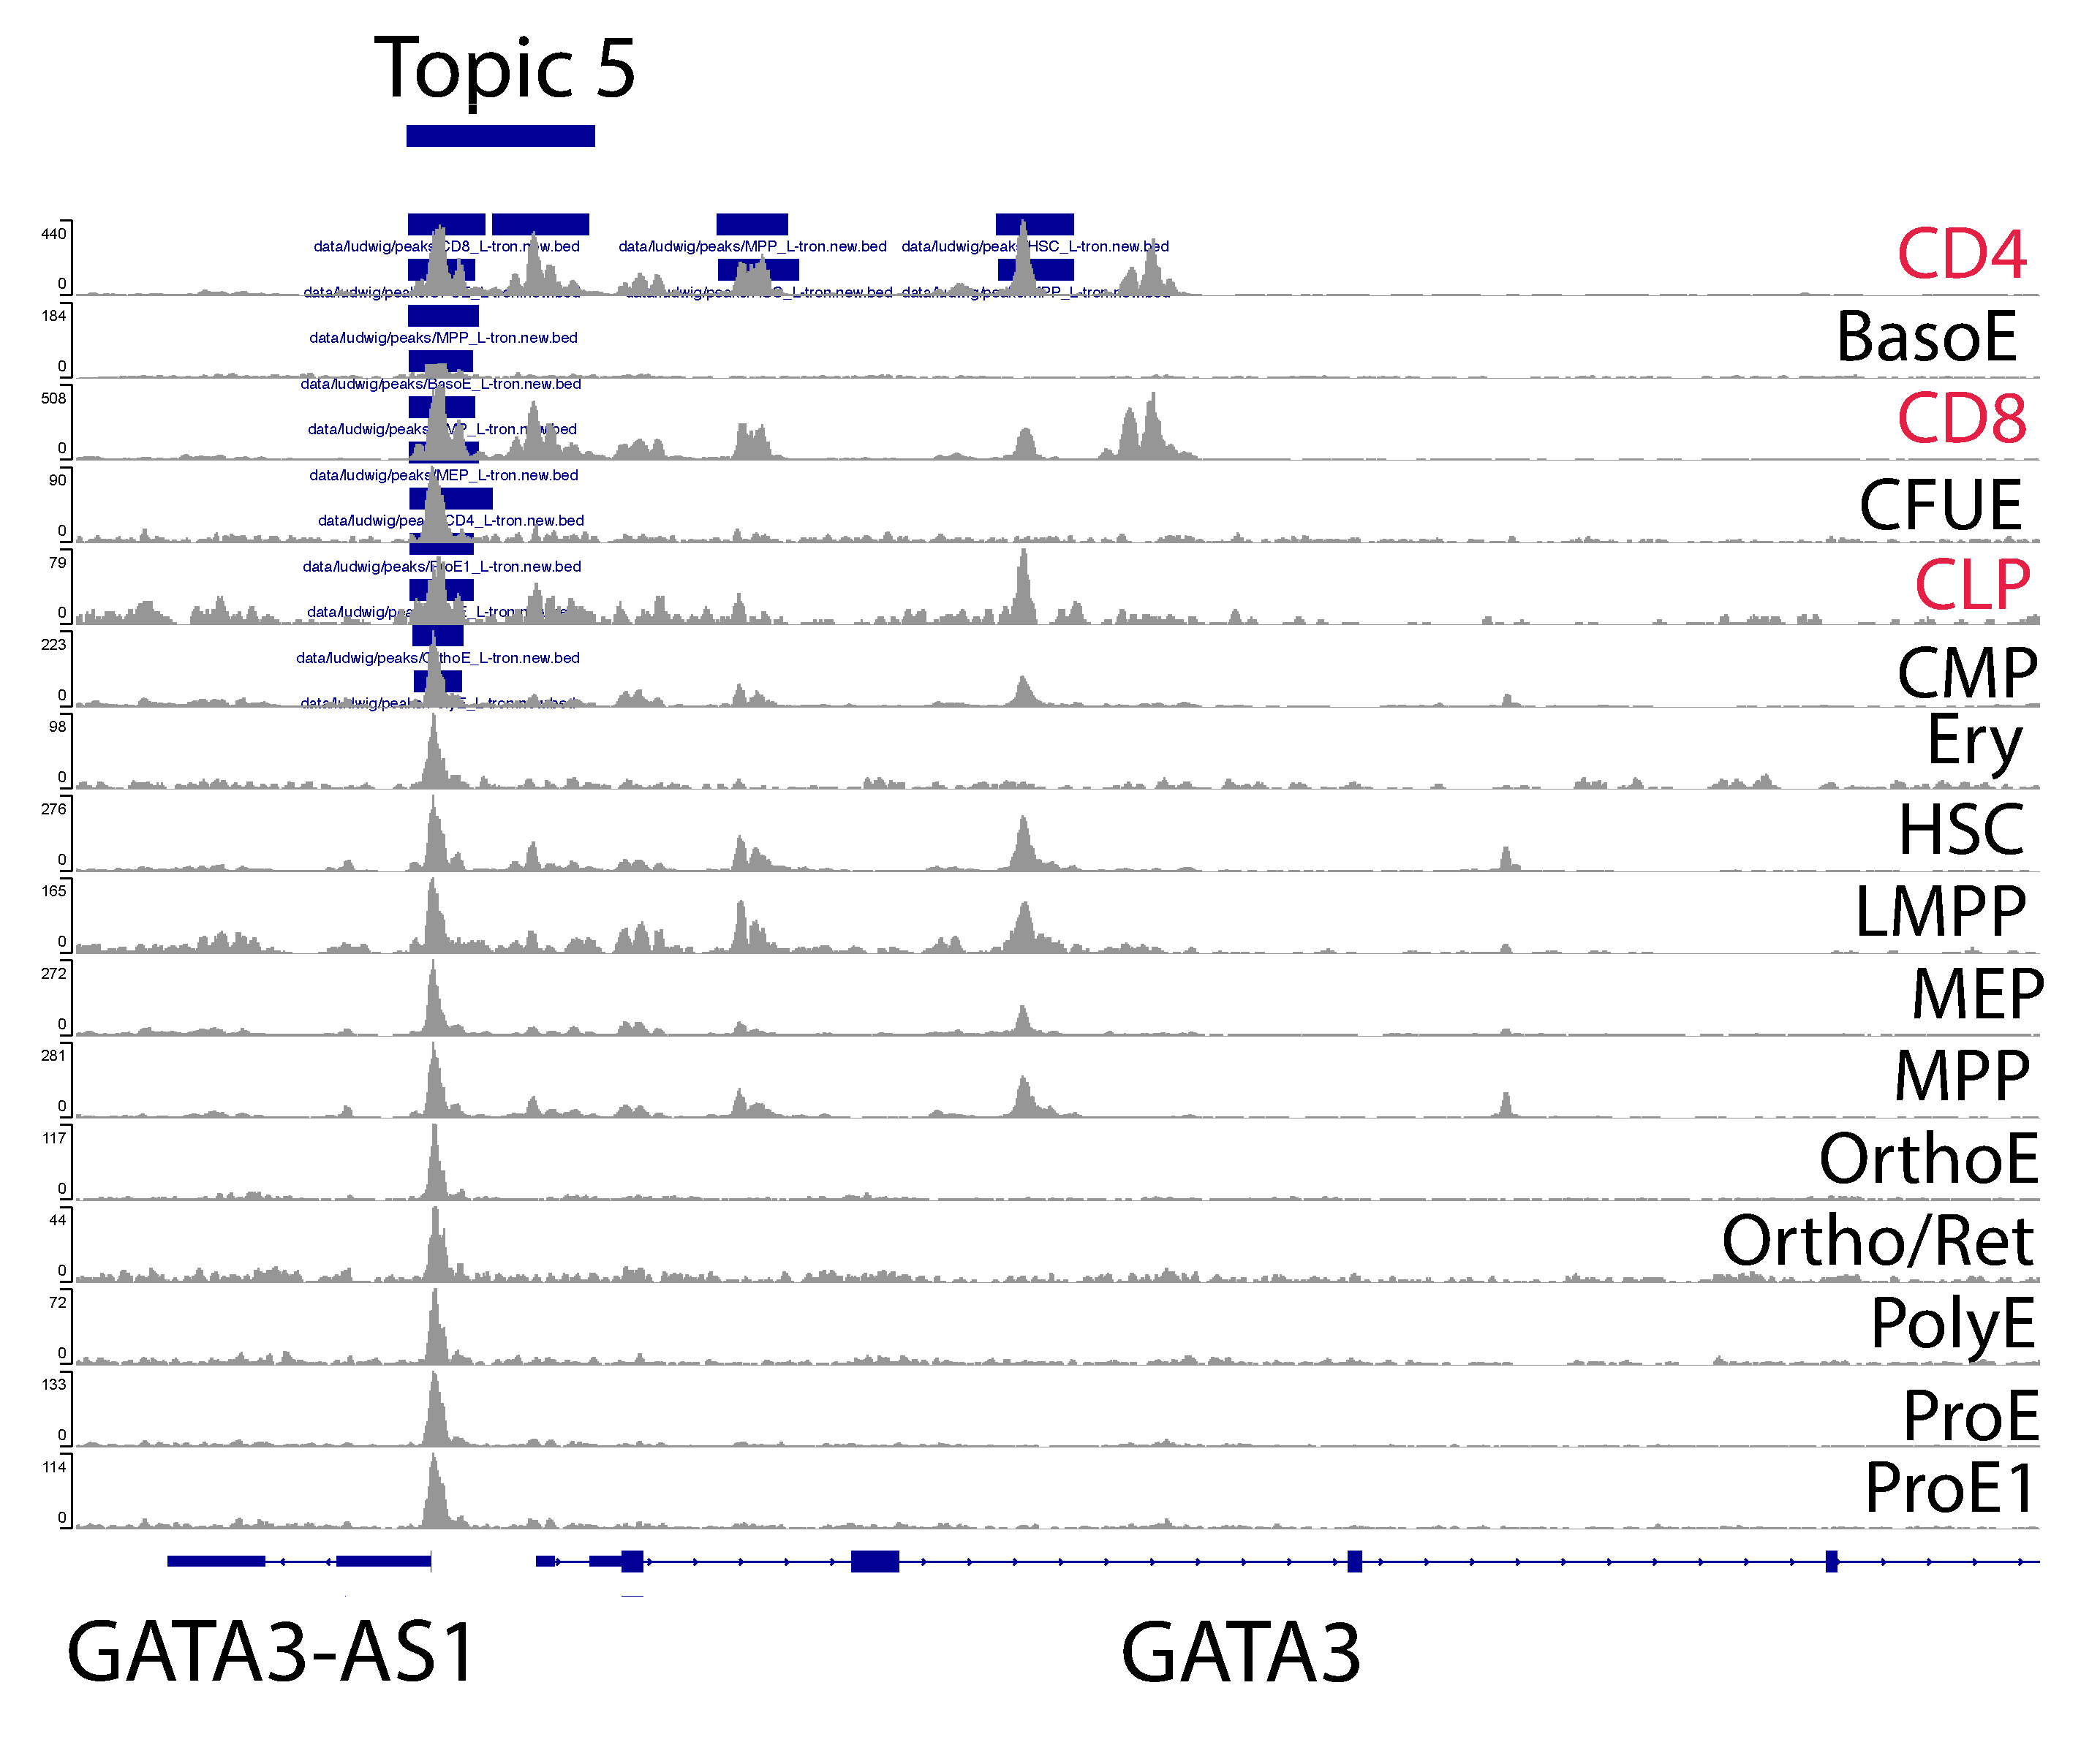
\includegraphics[width=\textwidth]{plot/ch4/GATA3.pdf}
  \caption[GATA3 Promotor]{Coverage plot of the GATA3 promoter. BLDA identifies this region as discremintory for CD4 and CD8 T cells, and coverage plot indicates that it is differentially accessible between erythopoetic and terminally differentiated lymphocytes.}
  \todo{Why is the other beds peaking through???}
  \label{fig:gata3}
\end{figure}


Topic 1:
  - Stat5a promotor is one of the most important regions. Stat5a is 
    -  regulation of RBC production by expansion of earlier progenitor and stem cell populations.
    - topic 1 esxpression starts early and ramps up through erythropoesis
    - (and 2) share a peak with MiR584. What role does this play?

  Topic 8 (and 5)
    - CGAS is widely expressed but especially in hematopoetic progeneitors (https://www.frontiersin.org/articles/10.3389/fimmu.2020.573915/full)

Topic 2
  - Many of the systems like UROS, CCND3, VEGFA, and TMCC2 are not found in this system.
  - RHAG is found, peak accessibility in BasoE and the topic it is found in peaks with BaseO. 
  - HDAC6, some role in enucleation,not completelysure (https://www.ncbi.nlm.nih.gov/pmc/articles/PMC5451330/)

Topic5:
  - Has a promotor for GATA3. Maybe because this is not accessible in CD8 and CD4? But in everything else? 
    - Motifs found in almsot every other cell type
  - Actually also important for t cells https://www.ncbi.nlm.nih.gov/pmc/articles/PMC3688666/

Early: 
  - Arid3a / bright (6)
  - MEIS1 is expressed prefernetially in HSCs (https://www.ncbi.nlm.nih.gov/pmc/articles/PMC3525022/)
